\documentclass{article}
\usepackage[a4paper, margin=3mm, landscape]{geometry}
\usepackage{multicol}
\usepackage{xcolor}
\usepackage{enumitem}
\usepackage{amsmath}
\usepackage{amsfonts}
\usepackage{listings}
\usepackage{soul}
\usepackage{graphicx}

\pdfinfo{
    /Title (ST2334.pdf)
    /Creator (TeX)
    /Producer (pdfTeX 1.40.0)
    /Author (Jason Qiu)
    /Subject (ST2334)
    /Keywords (ST2334, nus, cheatsheet,pdf)
}

\graphicspath{ {./img/} }

\pagestyle{empty}
\setcounter{secnumdepth}{0}
\setlength{\columnseprule}{0.25pt}

% Redefine section commands to use less space
\makeatletter
\renewcommand{\section}{\@startsection{section}{1}{0mm}%
    {-1ex plus -.5ex minus -.2ex}%
    {0.5ex plus .2ex}%x
{\normalfont\large\bfseries}}
\renewcommand{\subsection}{\@startsection{subsection}{2}{0mm}%
    {-1explus -.5ex minus -.2ex}%
    {0.5ex plus .2ex}%
{\normalfont\normalsize\bfseries}}
\renewcommand{\subsubsection}{\@startsection{subsubsection}{3}{0mm}%
    {-1ex plus -.5ex minus -.2ex}%
    {1ex plus .2ex}%
{\normalfont\small\bfseries}}%
\makeatother

% Adjust spacing for all itemize/enumerate
\setlength{\leftmargini}{0.5cm}
\setlength{\leftmarginii}{0.5cm}
\setlist[itemize,1]{leftmargin=2mm,labelindent=1mm,labelsep=1mm}
\setlist[itemize,2]{leftmargin=2mm,labelindent=1mm,labelsep=1mm,label=$\bullet$}

% Font
\renewcommand{\familydefault}{\sfdefault}

% Define colors for math formulas
\definecolor{myblue}{cmyk}{1,.72,0,.38}
\everymath\expandafter{\the\everymath \color{myblue}}

% Custom command for keywords
\definecolor{highlight}{RGB}{251,243,218}
\newcommand{\keyword}[2][]{\sethlcolor{highlight}\hl{\textbf{#2}} #1 - }
\newcommand{\ilkeyword}[1]{\sethlcolor{highlight}\hl{\textbf{#1}}}

% Define colors and style for code
\definecolor{codegreen}{rgb}{0,0.6,0}
\definecolor{codegray}{rgb}{0.5,0.5,0.5}
\definecolor{codered}{HTML}{CC241D}
\definecolor{backcolor}{rgb}{0.95,0.95,0.95}
\lstdefinestyle{codestyle}{
    backgroundcolor = \color{backcolor},
    commentstyle = \color{codegray},
    keywordstyle = \color{codered},
    stringstyle = \color{codegreen},
    basicstyle = \ttfamily,
    breakatwhitespace = false,
    showstringspaces = false,
    breaklines = true,
    showtabs = false,
    tabsize = 2
}
\lstset{style = codestyle}

% -----------------------------------------------------------------------
\begin{document}
\begin{multicols*}{3}
\footnotesize

% Title box
\begin{center}
    \fbox{
        \parbox{0.8\linewidth}{
            \centering \textcolor{black}{
                {\Large\textbf{ST2334}} \\
                \normalsize{AY22/23 Sem 1}} \\
                {\footnotesize \textcolor{gray}{github.com/jasonqiu212}}
        }
    }
\end{center}

\section{01. Basic Concepts of Probability}

\subsection{Event Operations}

\begin{itemize}
    \item \keyword{Mututally Exclusive}{$A \cap B = \emptyset$}
    \item \keyword{Contained}{$A \subset B$}
    \item \keyword{Equivalence}{$A \subset B$ and $A \supset B \rightarrow A = B$}
    \item \keyword{Distributive}{$A \cap (B \cup C) = (A \cup B) \cup (A \cup C)$}
    \item \keyword{DeMorgan's}{$(A \cup B)' = A' \cap B'$}
    \item $A = (A \cap B) \cup (A \cap B')$
\end{itemize}

\subsection{Counting Methods}

\begin{itemize}
    \item \keyword{Multiplcation Principle}{Given r experiments performed \textbf{sequentially} and each has $n_1, n_2, \cdots, n_r$ outcomes. After r experiments, there are $n_1 n_2 \cdots n_r$ outcomes.}
    \item \keyword{Addition Principle}{Given experiment can be done in k different ways and each has $n_1, n_2, \cdots, n_r$ ways. There are $n_1 + n_2 + \cdots + n_k$ total ways.}
    \item \keyword{Permutation}{$_{n}P_{r} = \frac{n!}{(n-r)!}$}
    \item \keyword{Combination}{$\binom{n}{r} = \frac{n!}{(n-r)!r!}$}
\end{itemize}

\subsection{Probability}

\subsubsection{Axioms of Probability}
\begin{enumerate}
    \item For any event A, $0 \leq P(A) \leq 1$
    \item P(S) = 1
    \item If $A \cap B = \emptyset$, then $P(A \cup B) = P(A) + P(B)$
\end{enumerate}
\begin{itemize}
    \item $P(A') = 1 - P(A)$
    \item $P(A) = P(A \cap B) + P(A \cap B')$
    \item $P(A \cup B) = P(A) + P(B) - P(A \cap B)$
    \item If $A \subset B$, then $P(A) < P(B)$
\end{itemize}

\subsection{Finite Sample Space with Equally Likely Outcomes}

Given sample space $S = \{a_1, \cdots, a_k\}$ and all outcomes are \textbf{equally likely}, i.e. $P(a_1) = \cdots = P(a_k)$:
\[\text{For any event } A \subset S, P(A) = \frac{\text{No. of sample points in A}}{\text{No. of sample points in S}}\]

\subsection{Conditional Probability}

\[P(B|A) = \frac{P(B \cap A)}{P(A)} = \frac{P(A|B)P(B)}{P(A)}\]

\subsection{Independence}

\begin{itemize}
    \item $A \perp B \leftrightarrow P(A \cap B) = P(A)P(B)$
    \item $A \perp B \leftrightarrow P(A|B) = P(A)$
\end{itemize}

\subsection{Law of Total Probability}

\begin{itemize}
    \item \keyword{Partition}{If $A_1, \cdots, A_n$ are mutually exclusive events and $\bigcup _{i=1} ^{n} A_i = S$, then $A_1, \cdots, A_n$ are partitions}
    \item If $A_1, \cdots, A_n$ are partitions of S, then for any event B:
    \[P(B) = \sum _{i=1} ^{n} P(B \cap A_i) = \sum _{i=1} ^{n} P(B|A_i)P(A_i)\]
\end{itemize}

\subsection{Bayes' Theorem}

Let $A_1, \cdots, A_n$ be partitions of S. For any event B:
\[P(A_k|B) = \frac{P(B|A_k)P(A_k)}{\sum _{i=1} ^{n} P(B|A_k)P(A_i)}\]

\section{02. Random Variables}

\begin{itemize}
    \item Motivation: Assign value to outcome of experiment
    \item \keyword{Random Variable}{Let S be sample space. Function X which maps $\mathbb{R}$ to every $s \in S$}
\end{itemize}

\subsection{Probability Distribution}

\begin{itemize}
    \item Probability assigned to each possible $X$
    \item Given RV $X$ with range of $R_x$:
        \subitem \keyword{Discrete}{Numbers in $R_x$ are finite or countable}
        \subitem \keyword{Continuous}{$R_x$ is interval}
\end{itemize}

\subsubsection{Discrete Probability Distribution}
\begin{itemize}
    \item \keyword{Probability Function}{Given $R_x = \{x_1, \cdots\}$. For each $x_i$, there's some probability that $X = x_i$:}
    \[f(x) = P(X = x)\]
    \item $p.f.$ must satisfy:
        \begin{enumerate}
            \item $f(x_i) = P(X = x_i)$ for $x_i \in R_x$
            \item $f(x_i) = 0$ for $x_i \notin R_x$
            \item $\sum _{i=1} ^{\infty} f(x_i) = 1$
            \item $\forall B \subseteq \mathbb{R}, P(X \in B) = \sum _{x_i \in B \cap R_x} f(x_i)$
        \end{enumerate}
    \item \keyword{Probability Distribution}{Collection of pairs $(x_i, f(x_i))$}
\end{itemize}

\subsubsection{Continuous Probability Distribution}
\begin{itemize}
    \item \keyword{Probability Function}{Given $R_x$ is interval. Quantifies probability that $X$ is in some range.}
    \item $p.f.$ must satisfy:
        \begin{enumerate}
            \item $f(x) \geq 0$
            \item $f(x) = 0$ for $x \notin R_x$
            \item $\int _{R_x} f(x) dx = 1$
            \item $\forall a,b \text{ s.t. } a \leq b, P(a \leq X \leq b) = \int _{a} ^{b} f(x) dx$
        \end{enumerate}
    \item Note: $P(X = x_0) = \int _{x_0} ^{x_0} f(x) dx = 0$
\end{itemize}

\subsection{Cumulative Distributive Function}

Given RV $X$, which can be discrete or continuous:
\[F(x) = P(X \leq x)\]

\begin{itemize}
    \item $F(x)$ is non-decreasing and $0 \leq F(x) \leq 1$
    \item \textbf{For discrete RV}: Step function
    \[F(x) = \sum _{t \in R_x; t \leq x} f(t)\]
    \begin{itemize}
        \item $P(a \leq X \leq b) = F(b) - \lim _{x \to a^-} F(x)$
        \item $0 \leq f(x) \leq 1$
    \end{itemize}

    \item \textbf{For continuous RV}:
    \[F(x) = \int _{-\infty} ^{x} f(t) dt\]
    \[f(x) = \frac{d(F(x))}{dx}\]
    \begin{itemize}
        \item $P(a \leq X \leq b) = P(a < X < b) = F(b) - F(a)$
        \item $0 \leq f(x)$ e.g. $f(x) = 3x^2$ is a valid $p.f.$ since $\int _{R_x} f(x) dx = 1$
    \end{itemize}
\end{itemize}

\subsection{Expectation of Random Variable}

\begin{itemize}
    \item \textbf{Mean of discrete RV}: 
    \[\mu = E(X) = \sum _{x \in R_x} x_i f(x_i) = \sum _{i=1} ^{\infty} P(X \geq i)\]
    \begin{itemize}
        \item Let $g$ be some function. $E(g(x)) = \sum _{x \in R_x} g(x)f(x)$
    \end{itemize}
    \item \textbf{Mean of continuous RV}: 
    \[\mu = E(X) = \int _{x \in R_x} x f(x) dx\]
    \begin{itemize}
        \item Let $g$ be some function. $E(g(x)) = \int _{x \in R_x} g(x)f(x)dx$
    \end{itemize}
    \item $E(aX + b) = aE(X) + b$
    \item Linearity of expectation: $E(X + Y) = E(X) + E(Y)$
\end{itemize}

\subsection{Variance of Random Variable}

\[\sigma_X^2 = V(X) = E((X - \mu_X)^2)\]

\begin{itemize}
    \item \textbf{Variance of discrete RV}: 
    \[V(X) = \sum _{x \in R_x} (x - \mu_X)^2 f(x)\]
    \item \textbf{Variance of continuous RV}: 
    \[V(X) = \int _{x \in R_x} (x - \mu_X)^2 f(x) dx\]
    \item $V(X) = 0$ when $X$ is a constant
    \item $V(aX+b) = a^2V(X)$
    \item $V(X) = E(X^2) - (E(X))^2$
    \item \keyword{Standard Deviation}{$\sigma_X = \sqrt{V(X)}$}
\end{itemize}

\section{03. Joint Distributions}

\begin{itemize}
    \item Motivation: What if interested in more than 1 RV simultaneously?
    \item Given sample space $S$. Let $X$ and $Y$ be functions mapping $s \in S \to \mathbb{R}$:
    \[(X, Y) \text{is 2D random vector}\]
    \[\text{Range space: } R_{X, Y} = \{(x,y) | x = X(s), y=Y(s), s \in S\}\]
    \item \keyword{Discrete 2D RV}{If no. of possible values of $(X(s), Y(s))$ are finite or countable}
    \item \keyword{Continuous 2D RV}{If no. of possible values of $(X(s), Y(s))$ can be any value in Euclidean space $\mathbb{R}^2$}
    \item If both $X$ and $Y$ are discrete/continuous, then $(X, Y)$ is discrete/countinuous.
\end{itemize}

\subsection{Joint Probability Function}

\begin{itemize}
    \item \textbf{For discrete}:
    \[f_{X,Y} (x,y) = P(X = x, Y = y)\]
    \begin{itemize}
        \item $f_{X,Y} (x,y) \geq 0$ for any $(x,y) \in R_{X,Y}$
        \item $f_{X,Y} (x,y) = 0$ for any $(x,y) \notin R_{X,Y}$
        \item $\sum _{i=1} ^{\infty} \sum _{j=1} ^{\infty} P(X = x_i, Y = y_i) = 1$
        \item Let $A \subseteq R_{X, Y}$. $P((X,Y) \in A) = \sum \sum _{(x,y) \in A} f_{X, Y}(x,y)$
    \end{itemize}
    \item \textbf{For continuous}:
    \[P(a \leq X \leq b, c \leq Y \leq d) = \int _a ^b \int _c ^d f_{X, Y} (x, y)dydx\]
    \begin{itemize}
        \item $f_{X,Y} (x,y) \geq 0$ for any $(x,y) \in R_{X,Y}$
        \item $f_{X,Y} (x,y) = 0$ for any $(x,y) \notin R_{X,Y}$
        \item $\int _{-\infty} ^{\infty} \int _{-\infty} ^{\infty} f_{X,Y} (x,y)dxdy = 1$
    \end{itemize}
\end{itemize}

\subsection{Marginal Probability Function}

Let $(X,Y)$ be a 2D RV with joint probability function $f_{X,Y} (x,y)$:
\[\text{If $Y$ is discrete, } f_X(x) = \sum _y f_{X,Y} (x,y)\]
\[\text{If $Y$ is continuous, } f_X(x) = \int _{-\infty} ^\infty f_{X,Y} (x,y)dy\]

\begin{itemize}
    \item $f_Y (y)$ defined similarly
    \item Intuition: Marginal distribution for $X$ ignores presence of $Y$
    \item $f_X(x)$ is a $p.f.$
\end{itemize}

\subsection{Conditional Distribution}

Let $(X,Y)$ be a 2D RV with joint probability function $f_{X,Y} (x,y)$. Then $\forall x$ s.t. $f_X(x) > 0$:
\[f_{Y|X} (y|x) = \frac{f_{X,Y}(x,y)}{f_X (x)}\]

\begin{itemize}
    \item Intuition: Distribution of $Y$ given $X = x$
    \item Only defined for $x$ s.t. $f_X(x) > 0$
    \item $f_{Y|X} (y|x)$ is a $p.f.$ if we fix $x$
    \item But, $f_{Y|X} (y|x)$ is not a $p.f.$ for $x$
    \item $P(Y \leq y | X = x) = \int _{-\infty} ^y f_{Y|X} (y|x)dy$
    \item $E(Y|X=x) = \int _{-\infty} ^{\infty} y f_{Y|X} (y|x)dy$
\end{itemize}

\subsection{Independent Random Variables}

\[X \perp Y \leftrightarrow \forall x,y, f_{X,Y} (x,y) = f_X (x) f_Y (y)\]

\begin{itemize}
    \item Necessary condition: $R_{X,Y}$ must be a product space. Else, dependent.
\end{itemize}

\subsubsection{Properties}
Suppose $X,Y$ are independent RV:
\begin{itemize}
    \item If $A,B \subseteq \mathbb{R}$, then events $X \in A$ and $Y \in B$ are independent:
    \[P(X \in A; Y \in B) = P(X \in A) P(Y \in B)\]
    \item $g_1(X)$ and $g_2(Y)$ are independent
    \item Independence is related with conditional distribution:
    \[f_X(x) > 0 \to f_{Y|X} (y|x) = f_Y(y)\]
    \[f_Y(y) > 0 \to f_{X|Y} (x|y) = f_X(x)\]
\end{itemize}

\subsubsection{Quick way to check independence}
\begin{enumerate}
    \item $R_{X,Y}$ is a product space. i.e. $R_X$ does not depend on $Y$ and vice versa.
    \item $f_{X,Y} (x,y)$ can be written as $cg_1(x)g_2(y)$ where $g_1$ depends on $x$ only and $g_2$ depends on $y$ only.
    \item For discrete: $f_X (x) = \frac{g_1(x)}{\sum _{t \in R_X} g_1 (t)}$
    \item For continuous: $f_X (x) = \frac{g_1(x)}{\int _{t \in R_X} g_1 (t)dt}$
\end{enumerate}

\subsection{Expectation}

Given 2 variable function $g(x,y)$:
\[\text{If $(X,Y)$ is discrete, } E(g(X,Y)) = \sum _x \sum _y g(x,y) f_{X,Y} (x,y)\]
\[\text{If $(X,Y)$ is continuous, } E(g(X,Y)) = \int _{-\infty} ^\infty \int _{-\infty} ^\infty g(x,y) f_{X,Y} (x,y) dydx\]

\begin{itemize}
    \item $E(XY) = E(X)E(Y)$ if $X \perp Y$
\end{itemize}

\subsection{Covariance}

\[cov(X,Y) = E((X - E(X))(Y - E(Y)))\]
\[\text{If $(X,Y)$ is discrete, } cov(X,Y) = \sum _x \sum _y (x - \mu_X)(y - \mu_Y) f_{X,Y} (x,y)\]
\[\text{If $(X,Y)$ is cont., } cov(X,Y) = \int _{-\infty} ^\infty \int _{-\infty} ^\infty (x - \mu_X)(y - \mu_Y) f_{X,Y} (x,y)dxdy\]

\begin{itemize}
    \item $cov(X,Y) = E(XY) - E(X)E(Y)$
    \item $X \perp Y \to cov(X,Y) = 0$. But converse is not always true.
    \item $cov(aX+b, cY+d) = (ac) cov(X,Y)$
    \item $V(aX+bY) = a^2V(X) + b^2V(Y) + 2abcov(X,Y)$
    \item $X \perp Y \to V(X + Y) = V(X) + V(Y)$
\end{itemize}
\section{04. Special Probability Distributions}

\subsection{Discrete Uniform Distribution}

\begin{itemize}
    \item If $X$ has values $x_1, x_2, \cdots, x_k$ with \textbf{equal probability}
    \item $p.f.$: $f_X(x) = \frac{1}{k}$ where $x = x_1, \cdots, x_k$ and $0$ otherwise
    \item Expectation: $\mu_X = E(X) = \sum_{i = 1} ^{k} x_i f_X (x_i) = \frac{1}{k} \sum_{i=1} ^{k} x_i$
    \item Variance: $\sigma_X^2 = V(X) = E(X^2) - (E(X))^2 = \frac{1}{k} \sum_{i=1} ^{k} x_i^2 - \mu_X^2$
\end{itemize}

\subsection{Bernoulli}

\begin{itemize}
    \item \keyword{Bernoulli Trial}{Random experiment with 2 possible outcomes (success and failure)}
\end{itemize}

\subsubsection{Bernoulli Random Variable}
\begin{itemize}
    \item Number of successes in Bernoulli trial (Either 1 or 0)
    \item Let $0 \leq p \leq 1$ be the probability of success in Bernoulli trial
    \[ f_X (x) = P(X = x) = 
    \begin{cases}
        p & x = 1\\
        1 - p & x = 0\\
        0 & otherwise
    \end{cases}
    \]
    \item $f_X (x) = p^x (1-p)^{1-x}$ for $x=0$ or $1$
    \item Notation: $X \sim Ber(p)$ and $q = 1 - p$
    \item $\mu_X = E(X) = p$ and $\sigma_X^2 = V(X) = p(1-p)$
\end{itemize}

\subsubsection{Bernoulli Process}
\begin{itemize}
    \item Sequence of repeatedly performed \textbf{independent and identical} Ber. trials
    \item Generates sequence of \textbf{independet and identically distributed (i.i.d.)} Ber. RVs: $X_1, X_2, \cdots$
\end{itemize}

\subsection{Binomial Distribution}

\begin{itemize}
    \item \keyword{Binomial RV}{Counts the number of successes in n trials in a Ber. process}
    \item Given n trials with each trial having probability p of success: 
    \[P(X = x) = \binom{n}{x} p^x (1-p)^{n-x}\]
    \item Notation: $X \sim B(n, p)$
    \item $E(X) = np$ and $V(X) = np(1-p)$
\end{itemize}

\subsection{Negative Binomial Distribution}

\begin{itemize}
    \item Let X = Number of i.i.d. Bernoulli(p) trials until kth success occurs
    \[P(X = x) = \binom{x-1}{k-1} p^k (1-p)^{x-k}\]
    \item Notation: $X \sim NB(k, p)$
    \item $E(X) = \frac{1}{p}$ and $V(X) = \frac{(1-p)}{p^2}$
\end{itemize}

\subsubsection{Geometric Distribution}
\begin{itemize}
    \item Let X = Number of i.i.d. Bernoulli(p) trials until 1st success occurs
    \[P(X = x) = p (1-p)^{x-1}\]
    \item Notation: $X \sim G(p)$
    \item $E(X) = \frac{1}{p}$ and $V(X) = \frac{1-p}{p^2}$
\end{itemize}

\subsection{Poisson Distribution}
\begin{itemize}
    \item \keyword{Poisson RV}{Denotes number of events happening in \textbf{fixed period of time or fixed region}}
    \[P(X = k) = \frac{e^{-\lambda}\lambda^k}{k!}\]
    \item Notation: $X \sim Poisson(\lambda)$ where $\lambda > 0$ is expected number of occurrences during given period/region
    \item $E(X) = \lambda$ and $V(X) = \lambda$
\end{itemize}

\subsubsection{Poisson Process}
\begin{itemize}
    \item Continuous time process, where we count number of occurrences within some interval of time
    \item Given Poisson process with rate parameter $\alpha$:
    \begin{itemize}
        \item Expected number of occurrences in interval of length $T$ is $\alpha T$
        \item No simultaneous occurrences
        \item Number of occurrences in disjoint intervals are independent
    \end{itemize}
    \item Number of occurrences in any interval $T$ of Poisson process follows $Poisson(\alpha T)$ distribution
\end{itemize}

\subsubsection{Poisson Approximation of Binomial Distribution}
Let $X \sim B(n, p)$. Suppose $n \to \infty$ and $p \to 0$ s.t. $\lambda = np$ remains constant. Then $X \sim Poisson(\lambda)$ approximately.
\[\lim _{p \to 0; n \to \infty} P(X = x) = \frac{e^{-np} (np)^x}{x!}\]

\begin{itemize}
    \item Approximation is good when $n \geq 20$ and $p \leq 0.05$, or $n \geq 100$ and $np \leq 10$
\end{itemize}

\subsection{Continuous Uniform Distribution}

X follows uniform distribution over interval $(a,b)$ if $p.f.$ is given by:
\[f_X (x) = 
\begin{cases}
    \frac{1}{b-a} & a \leq x \leq b\\
    0 & otherwise
\end{cases}
\]

\begin{itemize}
    \item Notation: $X \sim U(a, b)$
    \item $E(X) = \frac{a+b}{2}$ and $V(X) = \frac{(b-a)^2}{12}$
    \item $c.d.f.$ is given by:
    \[F_X (x) = 
    \begin{cases}
        0 & x < a\\
        \frac{x-a}{b-a} & a \leq x \leq b\\
        1 & x > b
    \end{cases}
    \]
\end{itemize}

\subsection{Exponential Distribution}

X follows exponential distribution with parameter $\lambda > 0$ if $p.f.$ is given by:
\[f_x (x) = 
\begin{cases}
    \lambda e^{-\lambda x} & x \geq 0\\
    0 & x < 0
\end{cases}\]

\begin{itemize}
    \item Notation: $X \sim Exp(\lambda)$
    \item $E(X) = \frac{1}{\lambda}$ and $V(X) = \frac{1}{\lambda^2}$
    \item $c.d.f.$ is given by:
    \[F_X (x) = 
    \begin{cases}
        1 - e^{-\lambda x} & x > 0\\
        0 & x \leq 0\\
    \end{cases}
    \]
    \item Suppose $X$ has exponential distribution with parameter $\lambda > 0$. Then for any positive numbers $s$ and $t$, we have:
    \[P(X > s+t | X > s) = P(X > t)\]
\end{itemize}

\subsection{Normal Distribution}

X follows normal distribution with mean $\mu$ and variance $\sigma^2$ if $p.f.$ is given by:
\[f_X (x) = \frac{1}{\sqrt{2 \pi} \sigma}e^{-(x-\mu)^2 / (2 \sigma ^2)}\]

\begin{itemize}
    \item Notation: $X \sim N(\mu, \sigma^2)$
    \item $E(X) = \mu$ and $V(X) = \sigma^2$
    \item $p.f.$ is bell-shaped curve and symmetric about $x = \mu$
    \item Total area under curve is 1
    \item 2 normal curves are identical in shape if they have same $\sigma ^2$. They differ in location by $\mu_1 - \mu_2$.
    \item As $\sigma$ increases, curve becomes more spread out
    \item If $X \sigma N(\mu, \sigma^2)$ and let $Z = \frac{X - \mu}{\sigma}$
\end{itemize}

\subsubsection{Standardized Normal Distribution}
If $X \sim N(\mu, \sigma ^2)$ and let 
\[Z = \frac{X - \mu}{\sigma}\]
then $Z \sim N(0, 1)$

\begin{itemize}
    \item $E(Z) = 0$ and $V(Z) = 1$
    \item $p.f.$ is given by:
    \[f_Z (z) = \frac{1}{\sqrt{2 \pi}} e^{-z^2 / 2}\]
    \item Importance of standardizing normal distribution is that it allows us to use tables to find probabilities
    \item Let $X \sim N(\mu, \sigma^2)$. We can compute $P(x_1 < X < x_2)$ by standadization:
    \[x_1 < X < x_2 \leftrightarrow \frac{x_1 - \mu}{\sigma} < \frac{X - \mu}{\sigma} < \frac{x_2 - \mu}{\sigma}\]
    \item $c.d.f.$ is given by:
    \[\phi(z) = F_Z (z) = \int _{-\infty} ^{z} f_Z (z) = \frac{1}{\sqrt{2 \pi}}\int _{-\infty} ^{z} e^{-t^2 / 2} dt\]
    \item $P(Z \geq 0) = P(Z \leq 0) = \phi(0) = 0.5$
    \item For any $z$, $\phi(z) = P(Z \leq z) = P(Z \geq -z) = 1-\phi(-z)$
    \item $-Z \sim N(0, 1)$
    \item If $Z \sim N(0, 1)$, then $\sigma Z + \mu \sim N(\mu, \sigma^2)$
    \item \keyword{Upper Quantile}{Given $\alpha$ is upper-tail percentage. The $\alpha$th upper quantile is $x_\alpha$ that satisfies:}
    \[P(X \geq x_\alpha) = \alpha\]
    e.g. The 0.05th (upper) quantile of $Z \sim N(0,1)$ is 1.645, i.e. $z_{0.05} = 1.645$.
    \item $P(Z \geq z_\alpha) = P(Z \leq -z_\alpha) = \alpha$
    \item $\text{Upper } z_\alpha = \text{Lower } z_{1-\alpha}$
\end{itemize}

\subsubsection{Normal Approximation to Binomial Distribution}
Let $X \sim B(n, p)$, then as $n \to \infty$:
\[Z = \frac{X - E(X)}{\sqrt{V(X)}} = \frac{X - np}{\sqrt{np(1-p)}} \sim N(0, 1)\]

\begin{itemize}
    \item Approximation is good when $np > 5$ and $n(1-p) > 5$
\end{itemize}

\section{05. Sampling Distributions}

\subsection{Population and Sample}

\begin{itemize}
    \item Motivation: Infer something about population using sample
    \item \keyword{Population}{All possible observations of survey}
    \item \keyword{Sample}{Subset of population}
    \item Every observation can be numerical or categorical
    \item Finite population vs. Infinite population
\end{itemize}

\subsection{Random Sampling}

\begin{itemize}
    \item Motivation: We usually know what distribution the population belongs to, but we don't know the parameters of the distribution. We can use sample to estimate the parameters.
    \item \keyword{Simple Random Sample}{Given sample of size $n$, each sample has equal chance of being selected}
\end{itemize}

\subsubsection{SRS for Infinite Population}
Let $X$ be RV with $p.f.$ $f_X (x)$. Let $X_1, X_2, \cdots, X_n$ be independent random variables with same distribution as $X$. Then $X_1, X_2, \cdots, X_n$ is a simple random sample of size $n$. Joint probability function of $X_1, \cdots, X_n$:
\[f_{X_1, \cdots, X_n} (x_1, \cdots, x_n) = f_X (x_1) f_X (x_2) \cdots f_X (x_n)\]

\subsubsection{Sampling with Replacement}
\begin{itemize}
    \item Sampling with replacement from finite population is considered as sampling from infinite population
    \item Sample is random if:
    \begin{itemize}
        \item Every element in population has same probability
        \item Successive draws are independent
    \end{itemize}
\end{itemize}

\subsection{Sample Distribution of Sample Mean}

\begin{itemize}
    \item \keyword{Statistic}{Suppose random sample of $n$ observations is $X_1, X_2, \cdots, X_n$. A statistic is a function of $X_1, \cdots, X_n$}
    \item \keyword{Sample Mean}{}
    \[\bar{X} = \frac{1}{n} \sum _{i=1} ^n X_i\]
    \item \keyword{Sample Variance}{}
    \[S^2 = \frac{1}{n-1} \sum _{i=1} ^n (X_i - \bar{X})^2\]
    \item \textbf{Statistics are random variables}. We can look at distribution of statistics.
    \item \keyword{Sample Distribution}{Distribution of a statistic}
    \item Mean and variance of $\bar{X}:$
    \[E(\bar{X}) = \mu \text{ and } V(\bar{X}) = \frac{\sigma_X ^2}{n}\]
    Intuition: $\mu_X$ is some unknown constant. $\bar{X}$ guesses that. As $n$ increases, accuracy of $\bar{X}$ increases.
    \item \keyword{Standard Error}{Standard deviation of sampling distribution (e.g. $\sigma_{\bar{X}}$)}
    \item \keyword{Law of Large Numbers}{As $n$ increases, $\bar{X}$ converges to $\mu_X$. i.e. For any $\epsilon \in \mathbb{R}$:}
    \[P(|\bar{X} - \mu| > \epsilon) \to 0 \text{ as } n \to \infty\]
\end{itemize}

\subsection{Central Limit Theorem}

If $\bar{X}$ is mean of random sample of size $n$ from population with mean $\mu$ and variance $\sigma^2$, then as $n \to \infty$:
\[\bar{X} \sim N(\mu, \frac{\sigma^2}{n}) \text{ approximately}\]

\begin{itemize}
    \item Intuition: For a large $n$, $\bar{X}$ is approximately normally distributed.
    \item If random sample is from normal population, $\bar{X}$ is normally distributed no matter value of $n$
    \item If very skewed, CLT may not hold even with large $n$
\end{itemize}

\subsection{Other Sampling Distributions}

\subsubsection{$\chi^2$ Distribution}
\begin{itemize}
    \item Let $Z_1, \cdots, Z_n$ be $n$ independent and identically distributed standard normal RVs. A $\chi^2$ RV with $n$ degrees of freedom is defined as a RV with same distribution as $Z_1^2 + \cdots + Z_n^2$
    \item Notation: $\chi^2 (n)$ with $n$ degrees of freedom
    \item If $Y \sim \chi^2 (n)$, then $E(Y) = n$ and $V(Y) = 2n$
    \item For large $n$, $\chi^2 (n)$ is approximately $N(n,2n)$
    \item If $Y_1$ and $Y_2$ are independent $\chi^2$ RVs with $m$ and $n$ degrees of freedom respectively, then $Y_1 + Y_2$ is $\chi^2 (m+n)$
    \item $\chi^2$ is family of curves. All density functions have long right tail.
\end{itemize}

\subsubsection{Sampling Distribution of $S^2$}
\begin{itemize}
    \item $E(S^2) = \sigma^2$
\end{itemize}

\subsubsection{Sampling Distribution of $\frac{(n-1)S^2}{\sigma^2}$}
If $S^2$ is variance of random sample of size $n$ from normal population of variance $\sigma^2$, then:
\[\frac{(n-1)S^2}{\sigma^2} = \frac{\sum _{i=1} ^{n} (X_i - \bar{X})^2}{\sigma^2}\]
has $\chi^2 (n-1)$ distribution

\subsubsection{t-Distribution}
Suppose $Z \sim N(0, 1)$ and $U \sim \chi^2 (n)$. If $Z$ and $U$ are independent, then:
\[T = \frac{Z}{\sqrt{U/n}} \sim t(n)\]
where $t(n)$ is called t-distribution with $n$ degrees of freedom

\begin{itemize}
    \item t-Distribution approaches $N(0,1)$ as $n \to \infty$
    \item When $n \geq 30$, t-distribution is approximately normal
    \item If $T \sim t(n)$, then $E(T) = 0$ and $V(T) = \frac{n}{n-2}$ for $n > 2$
    \item Symmetric about vertical axis and resembles standard normal distribution
    \item If $X_1, \cdots, X_n$ are independent and identically distributed normal RVs with mean $\mu$ and variance $\sigma^2$, then:
    \[\frac{X - \mu}{S / \sqrt{n}} \sim t(n-1)\]
\end{itemize}

\subsubsection{F-Distribution}
Suppose $U \sim \chi^2 (m)$ and $V \sim \chi^2 (n)$. If $U_1$ and $U_2$ are independent, then:
\[F = \frac{U / m}{V / m} \sim F(m,n)\]
is called F-distribution with $(m,n)$ degrees of freedom

\begin{itemize}
    \item If $X \sim F(m,n)$, then 
    \[E(X) = \frac{n}{n-2} \text{ for } n > 2\] 
    and 
    \[V(X) = \frac{2n^2(m+n-2)}{m(n-2)^2(n-4)} \text{ for } n>4\]
    \item If $F \sim F(m,n)$, then $1/F \sim F(n,m)$
\end{itemize}

\section{06. Estimation}

\subsection{Point Estimation for Mean}

\begin{itemize}
    \item Single number to estimate population parameter
    \item \keyword{Point Estimator}{Formula that describes this calculation}
    \item \keyword{Point Estimate}{Result of point estimator}
    \item Notation: $\theta$ represents parameter of interest. $\theta$ can be $p$, $\mu$, $\sigma$, etc.
\end{itemize}

\subsubsection{Unbiased Estimator}
Let $\hat{\theta}$ be an estimator of $\theta$. Then $\hat{\theta}$ is unbiased if:
\[E(\hat{\theta}) = \theta\]

\subsubsection{Maximum Error of Estimate}
\begin{itemize}
    \item Motivation: Usually $\bar{X} \neq \mu$. So $\bar{X} - \mu$ measures difference between estimator and parameter
    \item Let $z_\alpha$ be $\alpha$th upper quantile of standard normal distribution $Z$. i.e. $P(Z > z_\alpha) = \alpha$
    \[P(-z_{\alpha/2} \leq \frac{\bar{X} - \mu}{\sigma / \sqrt{n}} \leq z_{\alpha/2}) = P(|\bar{X} - \mu| \leq z_{\alpha/2} \frac{\sigma}{\sqrt{n}}) = 1 - \alpha\]
    \item \keyword{Maximum Error of Estimate}{Given probability $1-\alpha$:}
    \[E = z_{\alpha / 2} \frac{\sigma}{\sqrt{n}}\]
\end{itemize}

\subsubsection{Determination of Sample Size}
Given probability $1-\alpha$ and maximum error $E$, what is the minimum sample size $n$?
\[n \geq (\frac{z_{\alpha/2} \sigma}{E})^2\]

\subsubsection{Different Cases}
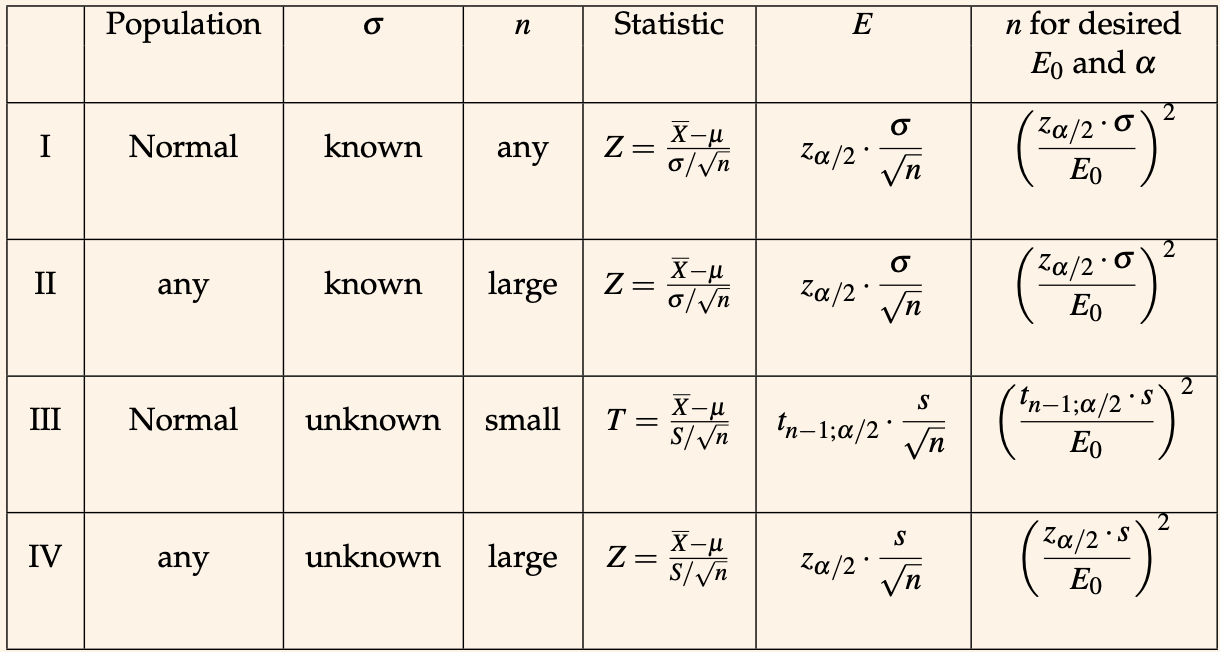
\includegraphics[scale=0.4]{point-estimation}

\subsection{Confidence Interval for Mean}

\begin{itemize}
    \item \keyword{Interval Estimator}{Rule for calculating an interval $(a,b)$ in which we are fairly certain the parameter lies}
    \item \keyword{Confidence Level}{Probability that interval contains parameter. i.e. $1 - \alpha$}
    \[P(a < \mu < b) = 1 - \alpha\]
    \item \keyword{Confidence Interval}{Interval calculated by interval estimator. i.e. $(a,b)$}
\end{itemize}

\subsubsection{Case 1: $\sigma$ known, data normal}
Previously:
\[P(-z_{\alpha/2} \leq \frac{\bar{X} - \mu}{\sigma / \sqrt{n}} \leq z_{a/2}) = 1 - \alpha\]
By rearranging, the $1 - \alpha$ confidence interval is:
\[(\bar{X} - z_{\alpha/2} \frac{\sigma}{\sqrt{n}}, \bar{X} + z_{\alpha/2} \frac{\sigma}{\sqrt{n}})\]

\subsubsection{Other Cases}
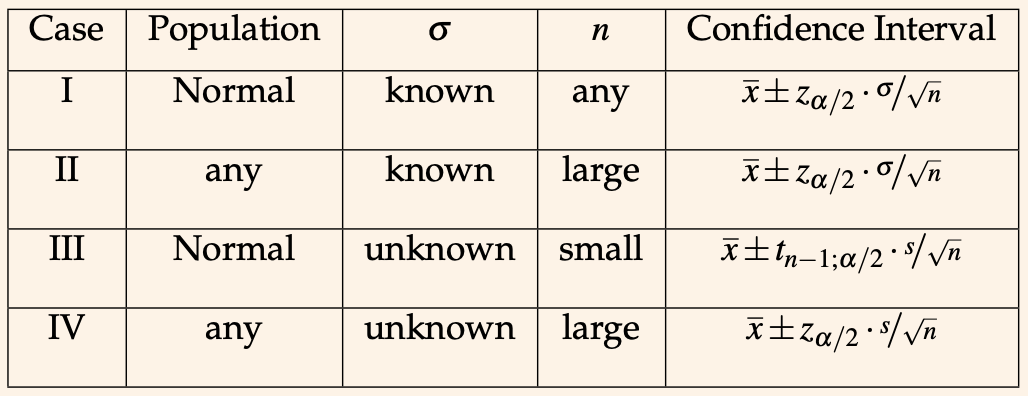
\includegraphics[scale=0.45]{confidence-interval}

\begin{itemize}
    \item $n$ is considered large when $n \geq 30$
\end{itemize}

\section{07. Hypothesis Testing}

\end{multicols*}
\end{document}
